\documentclass[bibliography=totoc, a4paper, 12pt]{scrreprt}
\usepackage[a4paper,left=1.5cm,right=1.5cm,top=1.5cm,bottom=1.5cm]{geometry}
\geometry{headheight=0.5cm, headsep=1.5cm, includehead}
\geometry{footskip=1.5cm ,includefoot}
\usepackage[ngerman]{babel}
\usepackage{caption}
\usepackage{booktabs}
\usepackage{graphicx} 
\usepackage[headsepline,footsepline, automark, autooneside=false, markcase=used]{scrlayer-scrpage}
\automark{chapter}
\usepackage[toc,page]{appendix}
\usepackage{blindtext}
\usepackage{acronym} % Abkürzungsverzichniss erstellen
\usepackage{enumitem}
\usepackage{tabularx}
\usepackage{enumitem}
\usepackage{ulem}
\usepackage[table]{xcolor}
\usepackage{xcolor,colortbl}
\usepackage{makecell} %for bigger lines in table
\usepackage{soul}
\usepackage{multicol}
\usepackage{multirow}
\usepackage{changepage}
\usepackage{ragged2e}
\usepackage{setspace} %Zeilenabstand
\usepackage{todonotes}
\usepackage{lineno}
\usepackage{amsmath} %Mathe to use equation
\usepackage{tikz}
\usetikzlibrary{arrows,automata,positioning}
\usepackage{pgfplots}
\usepackage{pdfpages}
\usepackage{makeidx} % fuer Stichwortverzeichnis 
\makeindex
\usepackage[hidelinks, pdfborder={0 0 0}, breaklinks]{hyperref}
%%-----------------------------------------------------------------------------------


%----------------------------------------------------------------------------------------
%						BibLaTex
\usepackage[backend=bibtex, style=numeric , citestyle=numeric , dateabbrev=false, sorting=none]{biblatex}
\addbibresource{sources.bib}
\DeclareFieldFormat{booktitle}{\newline{\textit{#1}}}%
\DeclareFieldFormat{url}{\newline URL: \url{#1}}%
\DeclareFieldFormat[inproceedings,standard,report]{title}{\newline #1}% Wenn der Titel zu lang wird kann mit, hier weiter Arten hinzufügen
\DeclareFieldFormat[misc]{note}{\newline #1}%

\renewcommand*{\labelnamepunct}{\addcolon\addspace}     % Semikollon nach Autor
\renewcommand*{\newunitpunct}{\addsemicolon\space} 		% Trennzeichen Semikolon
%----------------------------------------------------------------------------------------


\usepackage{listings}
\usepackage{color}

\author{author}

\ihead{Peer-to-Peer Volltextsuche}
\chead{Textextraktion-18}
\ohead{\headmark}
\cfoot{\\ Seite \pagemark}

\begin{document}
	\definecolor{mygreen}{rgb}{0,0.6,0}
\definecolor{mygray}{rgb}{0.5,0.5,0.5}
\definecolor{mylightgray}{rgb}{0.93,0.93,0.93}
\definecolor{mymauve}{rgb}{0.58,0,0.82}
\definecolor{darkblue}{rgb}{0.0,0.0,0.6}
\definecolor{cyan}{rgb}{0.0,0.6,0.6}
\definecolor{lightgray}{rgb}{.9,.9,.9}
\definecolor{darkgray}{rgb}{.4,.4,.4}
\definecolor{purple}{rgb}{0.65, 0.12, 0.82}
\definecolor{black}{rgb}{0,0,0}
\definecolor{white}{rgb}{1,1,1}
\definecolor{magicmint}{rgb}{0.67, 0.94, 0.82}

\lstset{ 
	backgroundcolor=\color{white},   % choose the background color; you must add \usepackage{color} or \usepackage{xcolor}; should come as last argument
	basicstyle=\footnotesize,        % the size of the fonts that are used for the code
	breakatwhitespace=false,         % sets if automatic breaks should only happen at whitespace
	breaklines=true,                 % sets automatic line breaking
	captionpos=t,                    % sets the caption-position to bottom
	commentstyle=\color{mygreen},    % comment style
	deletekeywords={...},            % if you want to delete keywords from the given language
	escapeinside={\%*}{*)},          % if you want to add LaTeX within your code
	extendedchars=true,              % lets you use non-ASCII characters; for 8-bits encodings only, does not work with UTF-8
	firstnumber=1,                % start line enumeration with line 1000
	frame=single,	                   % adds a frame around the code
	keepspaces=true,                 % keeps spaces in text, useful for keeping indentation of code (possibly needs columns=flexible)
	keywordstyle=\color{blue},       % keyword style
	morekeywords={*,...},            % if you want to add more keywords to the set
	numbers=left,                    % where to put the line-numbers; possible values are (none, left, right)
	numbersep=2pt,                   % how far the line-numbers are from the code
	numberstyle=\tiny\color{mygray}, % the style that is used for the line-numbers
	rulecolor=\color{black},         % if not set, the frame-color may be changed on line-breaks within not-black text (e.g. comments (green here))
	showspaces=false,                % show spaces everywhere adding particular underscores; it overrides 'showstringspaces'
	showstringspaces=false,          % underline spaces within strings only
	showtabs=false,                  % show tabs within strings adding particular underscores
	stepnumber=1,                    % the step between two line-numbers. If it's 1, each line will be numbered
	stringstyle=\color{mymauve},     % string literal style
	tabsize=2,	                   % sets default tabsize to 2 spaces
	title=\lstname,                   % show the filename of files included with \lstinputlisting; also try caption instead of title
	xleftmargin=2em,
	framexleftmargin=2em,
	literate=%
	{Ö}{{\"O}}1
	{Ä}{{\"A}}1
	{Ü}{{\"U}}1
	{ß}{{\ss}}1
	{ü}{{\"u}}1
	{ä}{{\"a}}1
	{ö}{{\"o}}1
	{~}{{\textasciitilde}}1
}
%----------------------------------------------------------------------------------------


\lstdefinestyle{customJava}{ %
  backgroundcolor=\color{white},   % choose the background color
  basicstyle=\footnotesize,        % size of fonts used for the code
  breaklines=true,                 % automatic line breaking only at whitespace
  commentstyle=\color{mygreen},    % comment style
  escapeinside={\%*}{*)},          % if you want to add LaTeX within your code
  keywordstyle=\color{blue},       % keyword style
  stringstyle=\color{mymauve},     % string literal style
  showspaces=false,
  showstringspaces=false,
  tabsize=2,
  numbers=left,
  stepnumber=1,
  frame=single,
  xleftmargin=2em,
  framexleftmargin=2em
}

\lstdefinelanguage{JavaScript}{
  keywords={break, case, catch, continue, debugger, default, delete, do, else, false, finally, for, function, if, in, instanceof, new, null, return, switch, this, throw, true, try, typeof, var, void, while, with},
  morecomment=[l]{//},
  morecomment=[s]{/*}{*/},
  morestring=[b]',
  morestring=[b]",
  ndkeywords={class, export, boolean, throw, implements, import, this},
  keywordstyle=\color{blue}\bfseries,
  ndkeywordstyle=\color{darkgray}\bfseries,
  identifierstyle=\color{black},
  commentstyle=\color{purple}\ttfamily,
  stringstyle=\color{red}\ttfamily,
  sensitive=true
}

\lstset{
   language=JavaScript,
   backgroundcolor=\color{lightgray},
   extendedchars=true,
   basicstyle=\footnotesize\ttfamily,
   showstringspaces=false,
   showspaces=false,
   numbers=left,
   numberstyle=\footnotesize,
   numbersep=9pt,
   tabsize=2,
   breaklines=true,
   showtabs=false
}

\lstdefinelanguage{Text}
{ 
	sensitive=false 
}

\lstdefinelanguage{XML}
{
  morestring=[b]",
  morestring=[s]{>}{<},
  morecomment=[s]{<?}{?>},
  stringstyle=\color{black},
  identifierstyle=\color{darkblue},
  keywordstyle=\color{cyan},
  morekeywords={xmlns,version,type}% list your attributes here
}
	%Tabellenlinie
\newcommand\btrule[1]{\specialrule{#1}{0pt}{0pt}}

%tabularx Gimmick
\newcolumntype{L}[1]{>{\raggedright\arraybackslash}p{#1}} % linksbündig mit Breitenangabe
\newcolumntype{C}[1]{>{\centering\arraybackslash}p{#1}} % zentriert mit Breitenangabe
\newcolumntype{R}[1]{>{\raggedleft\arraybackslash}p{#1}} % rechtsbündig mit Breitenangabe

%Tabellenheader White & Bold
\newcommand{\whitebf}[1]{\color{white}\textbf{\large#1}}

%Test in Anführungszeichen (german quote)
\newcommand{\gequote}[1]{\glqq #1\grqq{}}

%Auch bei chapter Header und Footer
\renewcommand*\chapterpagestyle{useheadings}

%Chapter Abstände
\renewcommand*\chapterheadstartvskip{\vspace*{-2.5\topskip}}
\renewcommand*\chapterheadendvskip{%
	\vspace*{1\baselineskip plus .1\baselineskip minus .167\baselineskip}}


%----------------------------------------------------------------------------------------
% 						Helping Commands
%
% \renewcommand{\arraystretch}{1.2} 	<- Tabelle strecken um 1.2 Punkte
% \rowcolors{1}{black!10}{black!1}		<- Tabellenzeilen haben verschiedene Farben
%
%----------------------------------------------------------------------------------------

%%-----------------------------------------------------------------------------------
\newcommand{\Todo}[1]{\todo[inline=true, linecolor=red,backgroundcolor=red!25,bordercolor=red]{#1}}
\newcommand{\Info}[1]{\todo[inline=true, linecolor=green,backgroundcolor=green!25,bordercolor=green]{#1}}
%%-----------------------------------------------------------------------------------

\newcommand{\tablehead}[2]{\rowcolor{magicmint}\multicolumn{#1}{|c|}{#2}}
\newcommand{\foreign}[1]{\dashuline{#1}}

\newcommand{\iitem}[1]{\item[...]\textit{#1}}
\newcommand{\iuitem}[1]{\item \textit{\uline{#1}}}

\newcommand{\mn}[2]{%
	\tikz [remember picture, baseline = (#1.base)]
	\node [inner sep = 0pt, outer sep = 2mm] (#1)
	{#2};
}
	
\newcommand{\cul}[3][black]{\xpatchcmd{\uline}
	{\bgroup}
	{\bgroup\def\ULthickness{2pt}}
	{}{}
	{\color{#2}\uline{{\color{#1}#3}}}} %<- Farbig unterschrichen und farbiger Text %\linenumbers
	\chapter{Ansatz}
Die inhaltliche Aufgabe der \textit{Textextraktion-18} war es alle Reden der 1. - 18. Wahlperiode zu extrahierten, hierbei sollten die vom \textit{Crawler} übergebenen XML-Dokumente extrahiert und in JSON Dateien ausgeben werden. Der \textit{Crawler} realisierte dies, durch die temporäre Persistierung der Plenarprotokolle als XML Dateien\cite{protokolle} und Übergabe als Parameter an die \textit{Textextraktion-18}.\\

\noindent Gegensatz zu den Plenarprotokollen der 19. Legislaturperiode liegen die Protokolle der 18. Legislaturperiode nicht in reinem XML Format vor (siehe \autoref{img:xml_begin_tags}), sondern es gibt am Anfang der XML Dateien die nötigsten XML Tags und das Protokoll selbst befindet sich in einem einzigen großen Textblock.
\begin{figure}[h]
	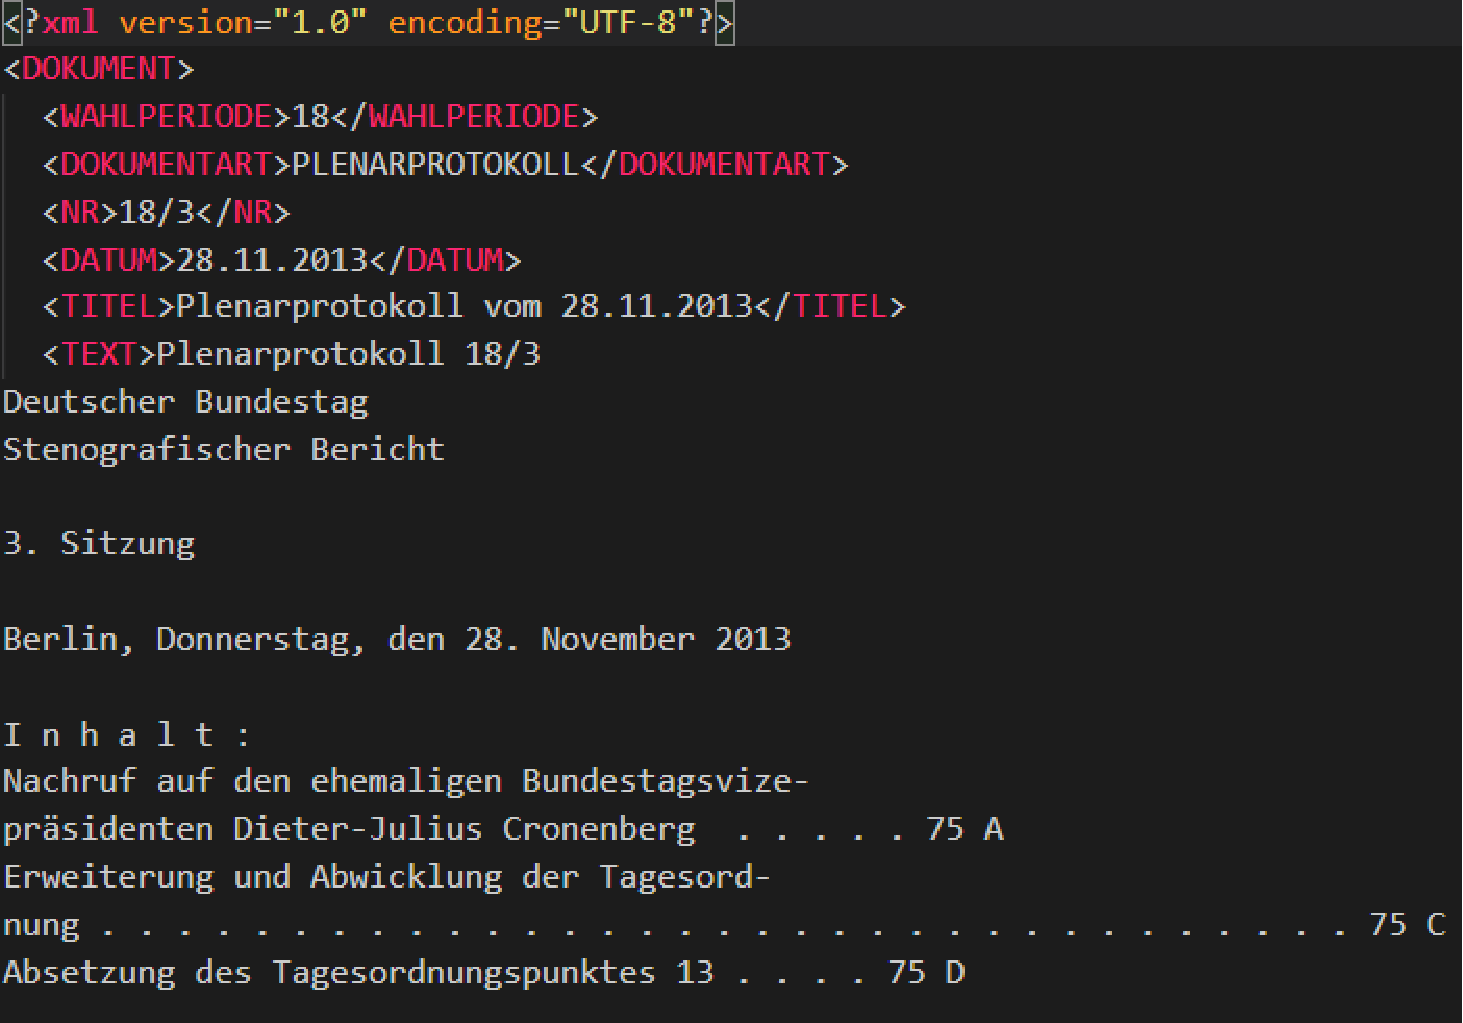
\includegraphics[width=\linewidth]{img/xml_begin_tags.pdf}
	\caption{18003.xml}
	\label{img:xml_begin_tags}
\end{figure}\\
Die Grundidee war nun also den Textblock semantisch und syntaktisch zu Untersuchen um einen Suchalgorithmus zu finden, welcher innerhalb des Textblockes:
\begin{multicols}{3}
	\begin{itemize}
		\item Titel der Rede
		\item Name des Sprechenden
		\item Zugehörigkeit
		\item Datum
		\item Rede
	\end{itemize}
\end{multicols}
zu einer Person findet und extrahiert.
	\chapter{Lösungsansatz}
\label{ch:solution}
Bei den Dokumenten handelt es sich um stenografische Berichte des deutschen Bundestages, weswegen angenommen wurde das alle Dokumente eine Konsistenz in der Formatierung des Textblockes besitzen. Somit befasste sich das Teilprojekt \textit{Textextraktion-18} vorerst mit der Extraktion eines Dokumentes, beispielhaft sollte dies das XML-Dokument 18003.xml sein.
\section{Analyse der XML-Dokumente}
\subsection{Inhaltsverzeichnis}
\label{subsec:toc}
Bereits nach kurzer Analyse des Dokuments stellte sich eine Auffälligkeit innerhalb des Inhaltsverzeichnisses heraus. Alle Kapitel wurden mit ihrem Titel, dem dazugehörigem Abschnitt im Protokoll und den beteiligten Sprechern gelistet (siehe \autoref{img:toc}).
\begin{figure}[h]
	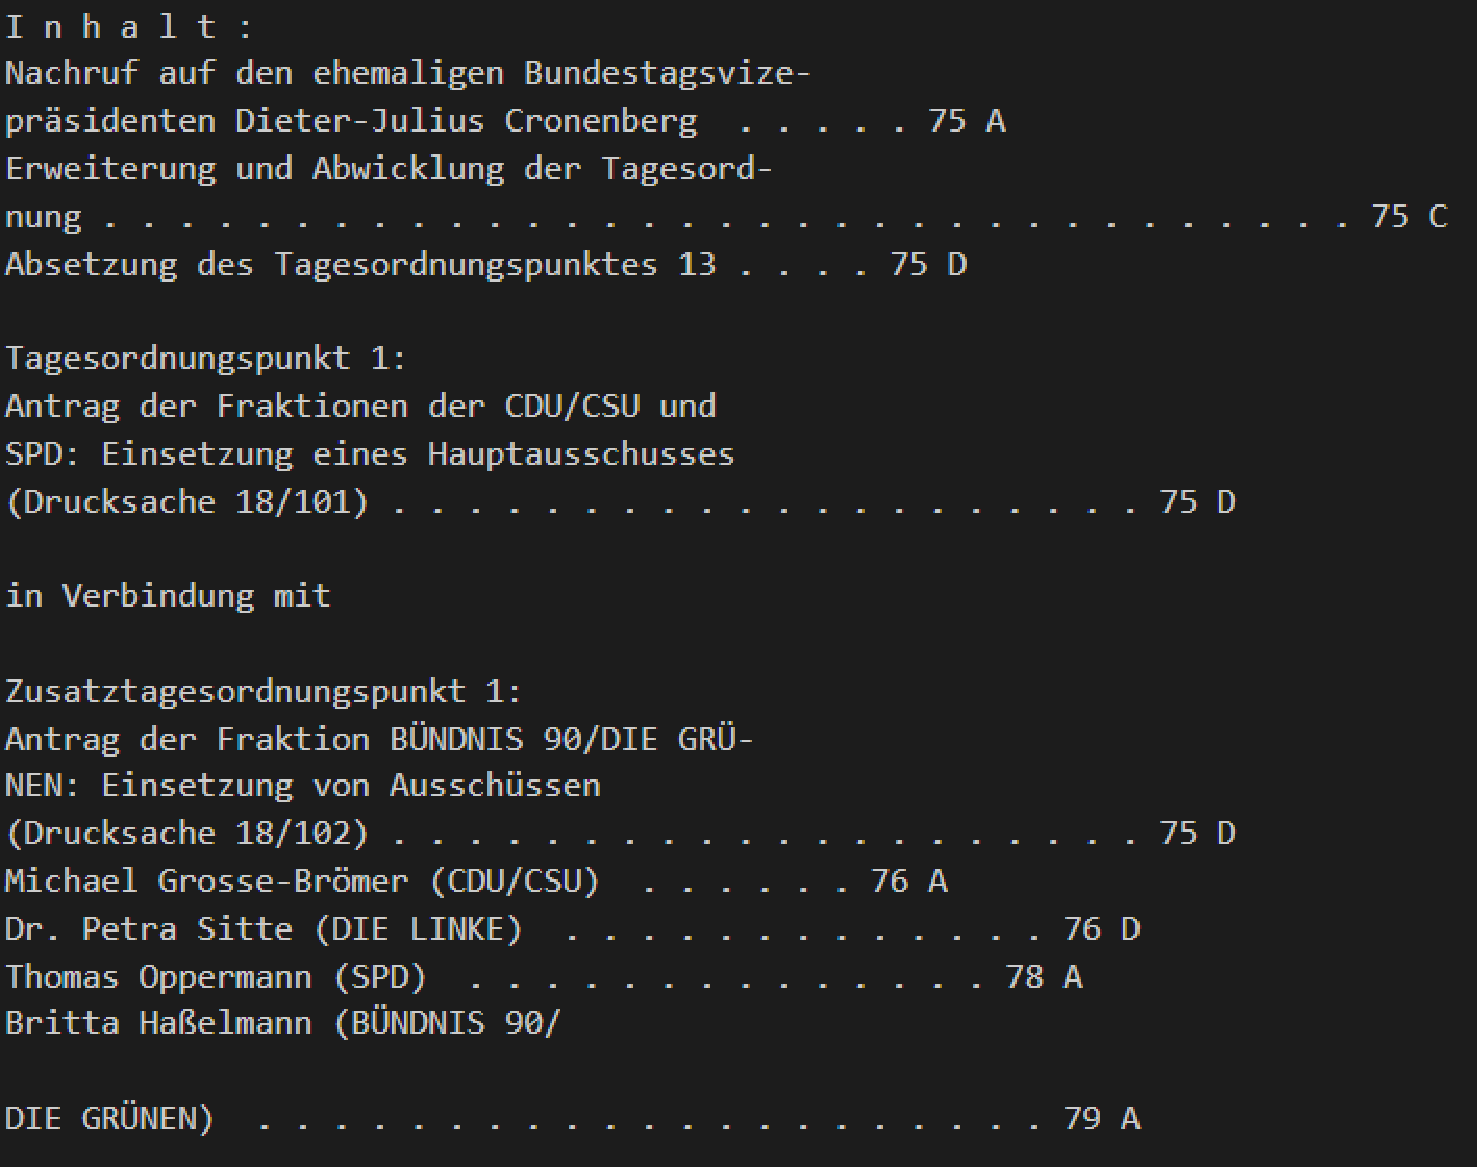
\includegraphics[width=\linewidth]{img/toc.pdf}
	\caption{Ansicht des Inhaltsverzeichnisses}
	\label{img:toc}
\end{figure}\newpage \noindent
\subsection{Eröffnungsrede}
\label{subsec:openning}
Zusätzlich wurde bei kurzem Vergleich mit wenigen anderen Dokumenten festgestellt, dass die Eröffnungsrede des Alterspräsident(siehe \autoref{img:begin}) scheinbar immer gleich eingeleitet wurde: \gequote{Beginn: 10.00 Uhr} (natürlich mit abweichender Uhrzeit)
\begin{figure}[h]
	\centering
	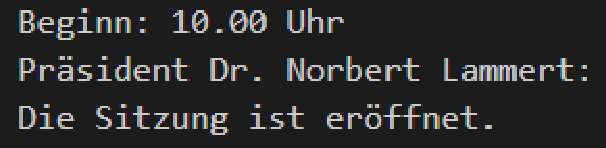
\includegraphics[width=.7\linewidth]{img/begin.pdf}
	\caption{Einleitung der Eröffnungsrede}
	\label{img:begin}
\end{figure}
\subsection{Redner}
\label{subsec:speech}
Darüber hinaus beginnt jede Rede mit dem Namen des Sprechenden und dessen Zugehörigkeit
\begin{figure}[h]
	\begin{minipage}{.42\linewidth}
		
\includegraphics[width=\linewidth]{img/petra.pdf}
	\end{minipage}\hfill
	\begin{minipage}{.54\linewidth}
		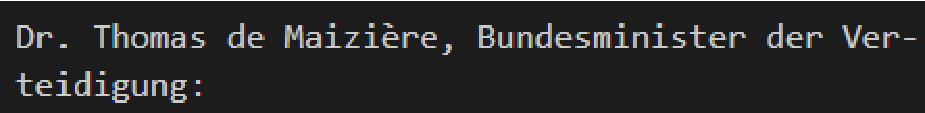
\includegraphics[width=\linewidth]{img/thomas.pdf}
	\end{minipage}
\end{figure}

\section{Extraktion mit Regulären Ausdrücken}
Es entwickelte sich die Idee anhand der Analyse reguläre Ausdrücke zu entwickeln die innerhalb des Textblockes passten (matchen). Für die einzelnen Teile der Analyse wurde dies wie folgt realisiert:
\begin{table}[h]
	\begin{tabularx}{\linewidth}{l X}
		\textbf{Analyseteil} & \textbf{regulärer Ausdruck}\\
		Inhaltsverzeichnis & \lstinline|TOC_NAMES = "\\d\\s[A-Z]\\n+"| \\
		Eröffnungsrede & \lstinline|OPENING = "(Uhr(\\r\|\\n\|(\\n)*)(?=(Vize\|Alters)?(P\|p)räsident(en\|in\|innen)?))"|\\
		Redner & \lstinline|BREAKINGPOINT = "(.+,\\s.+minister.+\\r*\\n*.+:\\n)\|((.+p\|P)räsident.+:\\n)\|(.+\\(.+\\):\\n)\|(.+\\(.+/.+-\\r*\\n*.+\\):\\n)\|(.+\\(.+\\r*\\n*.+\\):\\n)\|(.+,.+kanzler.+:\\n)"|\\
	\end{tabularx}
\end{table}

\newpage
\section{Theoretischer Ablauf}
Das zu erstellende Programm sollte nun grob wie folgt ablaufen:
\begin{enumerate}
	\item Einlesen des Dokuments, einzig relevante XML Tags sind \lstinline|<DATUM>| und \lstinline|<TEXT>|
	\item Alle Suchalgorithmen laufen innerhalb des Textblockes ab, das heißt im \lstinline|<TEXT>| Tag
	\item Durchsuche jeden Eintrag im Inhaltsverzeichnis nach Titeln und den dazugehörigen Rednern.
	\item Das Ende des Inhaltsverzeichnisses ist der Beginn der Eröffnungsrede des Alterspräsidenten.
	\item Alle nachträglichen Reden sollen dem Titel aus dem Inhaltsverzeichnis zugeordnet werden.
	\item Das Ende jeder Rede ist der Beginn einer neuen und kann mit dem \lstinline|BREAKINGPOINT| gefunden werden.
	\item Wurden alle Reden des Dokumentes gefunden sollen sie als JSON Datei gespeichert werden.
\end{enumerate}
	\chapter{Probleme}
	\chapter{Schlussbetrachtung}
Die grundlegende Anforderung alle Plenarprotokolle der 1.-18. Wahllegislaturperiode wurde in einem Sprint Review Meeting abgeändert, sodass vorrangig die Plenarprotokolle der 18. Wahllegislaturperiode extrahiert werden sollten.
Dieses Ziel wurde erreicht, allerdings gibt es Abstriche in Bezug auf die Form der einzelnen Bestandteile der extrahierten Reden im JSON Format.\\

\section{split versus substring}
In den ersten Versuchen wurden Strings, mithilfe von regulären Ausdrücken, in mindestens zwei Teile zerlegt. Dies hat allerdings zur Folge, dass nach mehreren solcher Zerlegungsprozesse ein Urzustand fast nicht mehr erreicht werden konnte. Daraus folgte die Benutzung von \lstinline|substring| welcher den Teilstring von Position X-Y zurückgibt ohne dessen Original zu überschreiben.

\section{Fazit}
Prinzipiell wurde innerhalb des Projektes eine spezifizierte KI geschrieben, welche Reden aus der 18. Wahllegislaturperiode anhand der frei zugänglichen XML-Dateien\cite{protokolle} verarbeitet und in JSON-Dateien umwandelt. Das Ergebnis ist verwertbar, kann aber noch verbessert werden in Bezug auf Performanz und Formatierung.\\
Alles in allem wurde das Projektziel erreicht und ist unter folgendem Link abrufbar:\\ \url{https://github.com/htw-projekt-p2p-volltextsuche/textextraction-18}
	
	\newpage
\clearscrheadings
\setheadsepline{0px}
\setfootsepline{0px}
\printbibliography[title={Quellenverzeichnis}]
\end{document}